%ATTENZIONE: PER COMPILARE BISOGNA FARE A MANO
%dvipdf tensor.dvi ;mv tensor.pdf temp.pdf 
%Dovremmo forse aggiungere due parole sulle C* algebras: non sono stateintrodotte proprio per evitare il tensor product in infinitedimensional systems?
%%%%%%%%%%%%%%%%%%%%%%%%%%%%%%%%%%%%%%%%%%%%%%%%%%%%%%%%%%%%%%%%%%%%%%%%
% The four postulates of quantum mechanics are three
%%%%%%%%%%%%%%%%%%%%%%%%%%%%%%%%%%%%%%%%%%%%%%%%%%%%%%%%%%%%%%%%%%%%%%%%
\documentclass[aps,prl,amsmath,amssymb,twocolumn]{revtex4}
%\documentclass[twocolumn,aps,showpacs,prl,groupedaddress]{revtex4}
%\usepackage{amssymb,stackengine}
\usepackage{amssymb}
\usepackage{color}
\usepackage{graphicx}
\usepackage{epsfig,amssymb,amsmath,amsthm}
%\usepackage[active]{srcltx}
%\usepackage[hypertex,linkcolor=red]{hyperref}

\usepackage{color}
\usepackage{cancel}
\usepackage{tikz-cd}

\theoremstyle{plain}
\newtheorem{thrm}{Theorem}[section]
\newtheorem{form}[thrm]{Formalization}
\newtheorem{prop}[thrm]{Proposition}
\newtheorem{lem}[thrm]{Lemma}

\theoremstyle{definition}
\newtheorem{defn}[thrm]{Definition}
\newtheorem{post}{Postulate}[]
\renewcommand*{\thepost}{(\alph{post})}

\theoremstyle{remark}
\newtheorem*{remark}{Remark}


\newcommand{\blue}{\color{blue}}  %NON LINEAR
\newcommand{\red}{\color{red}}
\newcommand{\cyan}{\color{cyan}}
\newcommand{\green}{\color{green}} %THEORY quantum state estimation
\newcommand{\yellow}{\color{yellow}} %THEORY quantum channel estimation

\DeclareMathOperator{\spn}{span}

\newcommand{\pj}[1] {\underbar{$#1$}}
%\newcommand{\pj}[1] {\overline{#1}}


\def\>{\rangle}
\def\<{\langle}
\def\ca{_{\cal A}}
\def\cb{_{\cal B}}
\def\cc{_{\cal C}}
\def\comment#1{}
%\def\comment#1{ [{\bf Comment Lor:} {\sf #1}]}
\def\commentg#1{ [{\bf Comment Gabriele:} {\sf #1}]}
\def\labell#1{\label{#1}}
%\def\labell#1{\label{#1}{\mbox{{\tiny #1}}}}
%\def\section#1{{\par\em #1:--- }}
\def\togli#1{}
\def\sh{\mbox{sh}}
\def\iden{\openone}
\begin{document}
	
	%\fbox{{\scriptsize Preprint. \today}}
	\title{The four postulates of quantum mechanics are three}
	\author{Gabriele Carcassi$^1$, Lorenzo Maccone$^{2}$ and Christine A. Aidala$^1$
	}\affiliation{\vbox{1.~Physics Department, University of Michigan, 450 Church Street,
			Ann Arbor, MI 48109-1040,
			United States}\\
		\vbox{2.~Dip.~Fisica and INFN Sez.\ Pavia, University
			of Pavia, via Bassi 6, I-27100 Pavia, Italy}}
	\begin{abstract}
		The tensor product postulate of quantum mechanics states that the
		Hilbert space of a composite system is the tensor product of the
		components' Hilbert spaces. All current formalizations of quantum
		mechanics that do not contain this postulate contain some equivalent
		postulate or assumption (sometimes hidden). Here we give a natural
		definition of composite system as a set containing the component
		systems and show how one can logically derive the tensor product
		rule from the state postulate and from the measurement postulate. In
		other words, our paper reduces by one the number of postulates
		necessary to quantum mechanics.
	\end{abstract}
	\pacs{}
	% Measurement theory (quantum mechanics), 03.65.Ta Mechanics quantum,
	% 03.65.-w noise quantum, 42.50.Lc quantum information, 03.67.Ac
	% Quantum information, 03.67.-a Quantum fluctuations, 42.50.Lc quantum
	% mechanics, 03.65.Ta quantum optics, 42.50.Gy
	\maketitle
	
	In this paper we derive the tensor product postulate (which, hence,
	loses its status of postulate) from two other postulates of quantum
	mechanics: the state postulate and the measurement postulate.
	The tensor product postulate does not appear in all axiomatizations of
	quantum mechanics: it has even been called ``postulate 0'' in some
	literature \cite{zurek}. A widespread belief is that it is a direct
	consequence of the superposition principle, and it is hence not a
	necessary axiom. {\em This belief is mistaken}: the superposition
	principle is encoded into the quantum axioms by requiring that the
	state space is a {\em linear} vector space. This is, by itself,
	insufficient to single out the tensor product, as other linear
	products of linear spaces exist, such as the direct product, the exterior/wedge product or the direct sum of vector spaces, which is used
	in classical mechanics to combine state spaces of linear systems. These are all maps from linear spaces to linear spaces but they differ in how the linearity of one is mapped to the linearity of the other.\footnote{For example, in the tensor product $a \otimes (b+c) = a \otimes b + a \otimes c$ while in the direct product $a \times (b+c) = a \times b + 0 \times c$ where $0$ is the zero vector. Also, in the tensor product $r  (a \otimes b) = (r a) \otimes b = a \otimes (r b)$ while in the direct product $r  (a \times b) = r a \times r b$, where $r$ is a scalar.}
	This belief may have arisen from the seminal book of Dirac
	\cite{diracbook}, who introduces tensor products (Chap.~20) by
	appealing to linearity. However, he adds the seemingly innocuous
	request that the product among spaces be distributive (rather,
	bilinear), which is equivalent to postulating tensor products (or
	linear functions of them). It is not an innocuous request. For
	example it does not hold where the composite vector space of two
	linear spaces is described by the direct product, e.g.~in classical
	mechanics, for two strings of a guitar: it is not distributive.
	[General classical systems, not only linear ones, are also composed
	through the direct product.] Of course, Dirac is not constructing an
	axiomatic formulation, so his `sleight of hand' can be forgiven. In
	contrast, von Neumann (\cite{vonneumannbook} Chap.~VI.2, also
	\cite{jauch}) introduces tensor products by noticing that this is a
	natural choice in the position representation of wave mechanics (where
	they were introduced in \cite{weyl,epr}), and then {\em explicitly
		postulates} them in general: ``This rule of transformation is
	correct in any case for the coordinate and momentum operators [...]
	and it conforms with the [observable axiom and its linearity
	principles], we therefore postulate them generally.''
	\cite{vonneumannbook}.  More mathematical or conceptually-oriented
	modern formulations (e.g.~\cite{ozawa,masanes,wootters,nielsenchuang})
	introduce this postulate explicitly.  An interesting alternative is
	provided in \cite{ballentinebook,ballentinepaper}: after introducing
	tensor products, Ballentine verifies a posteriori that they give the
	correct laws of composition of probabilities. Similarly, Peres uses
	relativistic locality \cite{peres}. While these procedures seemingly
	bypass the need to postulate the tensor product, they do not guarantee
	that this is the {\em only} possible way of introducing composite
	systems in quantum mechanics. In the framework of quantum logic,
	tensor products arise from some additional conditions \cite{matolcsi}
	which (in contrast to what is done here) are not connected to the
	other postulates. Similar approaches appear in \cite{marmo,aerts}
	where tensor products were obtained by specifying additional physical
	or mathematical requirements. \comment{ {\em Il resto della frase da spostare in supp material} In quantum field theory one tends to
		avoid problems connected with tensor products of infinite dimensional
		spaces by focusing on algebraic commutation structures,
		e.g.~\cite{giddins,roos}.  In particular, the recent MIP*=RE result
		\cite{mipre} implies that, in infinite dimensions, the tensor product
		is strictly less computationally powerful than the commutation
		structures, emphasizing the difference among these two structures, at
		least for the infinite-dimensional case. We will consider the
		non-relativistic setting here.}
	
	We start
	from the natural definition of a composite system as the set of two
	(or more) quantum systems. The composite system is therefore
	made of system $A$ {\em and} (joined with) system $B$ and {\em nothing else}.\footnote{Note that this does not exclude entangled states since they too are characterized by the observables and only the observables of the constituents.} The first key insight is that the first two postulates of quantum theory (introduced below) already assume that the preparation of one system is independent from the preparation of another (statistical independence). In fact, we cannot even talk about a system in the first place if we cannot characterize it independently. The second key insight is that, since all measurement
	outcomes and all states of the subsystems plus the composite live in the same probability space, we will automatically have a map $M$ that for a pair of subsystems' states gives us the composite state that corresponds to the statistically independent case. These insights are enough to characterize mathematically the state space of the composite: the linearity given by the Hilbert space, together with the fact that the composite system is fully described by the observables of $A$ and $B$, allows to extend the construction to the composite states that do not satisfy statistical independence (the entangled states). So the work consists of two interrelated efforts: a physical argument that starts from the first two postulates and leads to the necessary existence of the composition map $M$ and its properties together with a formal argument that shows how $M$ leads to the tensor product.
	
	\comment{mettere nel supplementary:	We will mainly focus on
		kine\-mati\-cal\-ly-inde\-pen\-dent systems, namely no superselection rules or
		other restrictions to the state space are present: it is possible to
		prepare each subsystem of a composite system in a state that is
		independent of the other systems (preparation independence).  This is
		the only case in which the tensor product can be properly employed: the Hilbert space of composite
		systems that have restrictions is {\em not} the tensor product of the
		component spaces, but a subspace of it (e.g.~the anti-symmetric
		subspace for fermions). Typically this is ignored in the literature,
		since the tensor product formalism is very convenient and is often
		used also in these cases, and superselection rules are typically avoidable \cite{susskind,zanardi,zanardilloyd}. }
	
	To make these arguments precise, we will need to use elements of projective geometry.
	If $\psi$ is a vector in our Hilbert space, the pure states is represented by the ray $\pj{\psi}$, which is the subspace spanned by $\psi$. This includes not only vectors with arbitrary phase, but also arbitrary modulus. The term ``ray'' can therefore be misleading since $\pj{\psi}$ is really a complex { \em plane }. In the same way, constraining the observable $X$ to a particular value $x_0$ means identifying the subspace spanned by all eigenstates such that $X | \psi \> = x_0 |\psi\>$. As we need to map states and observables between subsystems and composite system, the map $M$ derived from the probability space is really a map between subspaces, between the projective spaces. The technical work, then, is to show that the map $M$ on the projective spaces corresponds to a map $m$ on the vector spaces and that $m$ can be taken to be, without loss of generality, the tensor product.

	This is done by showing that preparation independence and
	statistical independence imply three conditions on the map $m$:
	(H1)~totality: the map is defined on all states of the subsystems;
	(H2)~bilinearity: the map is bilinear thanks to the fundamental
	theorem of projective geometry; (H3)~span surjectivity: the span of
	the image of map coincides with the full composite Hilbert space.  We
	then prove that, if these three conditions H1, H2 and H3 hold, then
	the map $m$ is the tensor product, namely the Hilbert space of the
	composite system is a tensor product of the components: the tensor
	product ``postulate'', which hence loses its status of a postulate. An
	overview of all these logical implications is given in
	Fig.~\ref{f:fig}. The rest of the paper contains the sketch of this
	argument. The supplementary material contains the mathematical details.
	
	%%BoundingBox: 45 418 630 588
	%(%old BoundingBox: 45 382 649 547)
	\begin{figure}[ht]
		\epsfxsize=1.\hsize\leavevmode\epsffile{fig.eps}
		%\includegraphics[width=\linewidth, trim={0.2in 5.8in 2.5in 0.1in}, clip=true]{fig.eps}
		\caption{Schematic depiction of the logical implications used
			in this paper. FTPG stands for ``Fundamental Theorem of Projective Geometry''.  \label{f:fig}}\end{figure}
	
	We start with the axiomatization of quantum mechanics based on the following
	postulates (e.g.~\cite{ozawa,masanes,wootters,nielsenchuang}): (a)~The pure state of a
	system is described by a ray $\pj{\psi}$ corresponding to a set of
	non-zero vectors $|\psi\>$ in a complex Hilbert space, and the
	system's observable properties are described by self-adjoint operators
	acting on that space; (b)~The probability that a measurement of a
	property $X$, described by the operator with spectral decomposition \comment{Normalizzare qui e in altri posti!}
	$\sum_{x,i}x|x_i\>\<x_i|$ ($i$ a degeneracy index), returns a value
	$x$ given that the system is in state $\pj{\psi}$ is
	$p(x|\psi)=\sum_i|\<\psi|x_i\>|^2$ (Born rule). (c)~The state
	space of a composite system is given by the tensor product of the
	spaces of the component systems; (d)~The time evolution of an isolated
	system is described by a unitary operator acting on a vector
	representing the system state, $|\psi({t})\>=U_{t}|\psi({t}=0)\>$ or,
	equivalently, by the Schr\"odinger equation. The rest of quantum
	theory can be derived from these axioms. While some axiomatizations
	introduce further postulates, we will be using only (a) and (b) to
	derive (c), so the above are sufficient for our aims.
	
	\togli{This axiomatization implicitly contains a definition of
		``quantum system'' which is crucial for what follows, so we need to
		clarify the assumptions that it contains. We will use the following
		definition for a quantum
		system\togli{$\stackon[1pt]={\mbox{\tiny
					def}}$}$\stackrel{\mbox{\tiny def}}=${\em ``a quantum degree
			of freedom with $d$ (possibly discrete, or continuous, infinite)
			mutually exclusive (commuting) values for each of its properties.
			Its mathematical description is through a Hilbert space of
			dimension $d$ which contains all the states that describe the
			values of its possible properties. In accordance with the
			postulate (a), these values correspond to a basis of the space,
			given by the eigenvectors of the observable corresponding to that
			property''}. \commentg{We may have to revise to be more clear.
			Where is this used?} }
	
	Note that we limit ourselves to
	kinemati\-cal\-ly-inde\-pen\-dent systems, where all state vectors
	$|\psi\>$ in the system's Hilbert space $\cal H$ describe a valid
	state, {\em unconditioned on anything else}. We call this condition ``preparation independence'' and it should be noted that the tensor product applies only in this case. For example, the composite system of two electrons is not the tensor product, rather the anti-symmetrized tensor product, precisely because the second electron cannot be prepared in the same state of the first. We note
	that restrictions due to superselection rules arise either from
	practical (not fundamental) limitations on the actions of the
	experimenter \cite{susskind,zanardi,zanardilloyd} or from the use of
	ill-defined quantum systems. In the example above, the field is the proper quantum system and the electrons are its excitations. \footnote{We
	emphasize that the kinematic independence is inequivalent to dynamical
	independence (or isolation).  Indeed if two systems interact, their
	interaction may lead to dynamical restrictions in the state spaces.
	Here we will not consider dynamical evolution, which is contained in
	postulate (d).}
	
	The definition of a composite system as containing {\em only} the
	collection of the subsystems means that any preparation of both
	subsystems independently must correspond to the preparation of the
	composite system. Since states are defined by postulate (a) as rays in
	the respective Hilbert spaces, there must exist a map $M : \pj{\cal A}
	\times \pj{\cal B } \to \pj{\cal C}$ that takes a pair of states for
	the subsystems ($\pj{\cal A}$ and $\pj{\cal B }$ represent the
	projective spaces and the Cartesian product is the set of all possible
	pairs) and returns a state in the projective space $\pj{\cal C}$ for
	the composite. To visualize the geometrical meaning of $M$ directly within the Hilbert spaces, given a ray (a complex plane) in each of $\cal A$ and $\cal B$, $M$ returns a ray (a complex plane) in $\cal C$.  Our final goal will be to find a map
	$m:{\cal A}\times{\cal B}\to{\cal C}$ that acts on vectors in the
	Hilbert spaces $\cal A$, $\cal B$ and $\cal C$ consistently with $M$. Namely,
	$\pj{m(a,b)}=M(\pj{a},\pj{b})$ where the underline sign indicates the
	elements in the projective space. Again geometrically, $m$ takes a vector in each of $\cal A$ and $\cal B$, and returns a vector in $\cal C$ and we want this to be consistent with $M$ such that vectors picked from the same rays will return vectors in the same ray. We will prove that the map $m$ is
	the tensor product. We focus on pure states here: the argument can be
	extended to mixed states using standard tools \cite{ballentine}.
	
	The map $M$ must be injective: as said above, different states of the
	subsystems must correspond, by definition of composite system, to
	different states of the composite. Moreover, preparation independence
	implies that $M$, and hence $m$, must be total maps (condition H1): each subsystem of
	the composite system can be independently prepared and gives rise to a
	state of the composite.  H1 is not sufficient
	to identify the tensor product: by itself it does not even guarantee
	that the map $m$ is linear.
	
	Postulate (b) contains the connection between quantum mechanics
	and probability theory. It must then implicitly contain the
	axiomatization of probability, e.g.~see
	\cite{ballentinepaper,ballentinebook,cox}. One of the axioms of
	probability theory (axiom 4 in \cite{ballentinepaper}) asserts that
	the joint probability of events $a$ and $b$ given $z$ is
	$p(a\wedge b|z)=p(a|z)\:p(b|z\wedge a)$. Consider $p(a \wedge b | \psi \wedge b)$ which represents the probability of measuring $a$ on system $A$ and $b$ on system $B$ having prepared system $A$ in $\psi$ and system $B$ in $b$. We have $p(a \wedge b | \psi \wedge b) = p(a | \psi \wedge b \wedge b) p(b | \psi \wedge b) = p(a | \psi \wedge b ) p(b | \psi \wedge b)$. The Born rule tells us that $p(a | \psi \wedge b) = |\<a|\psi\>|^2$ and that $p(b | \psi \wedge b) = |\<b|b\>|^2 = 1$, where $a$, $b$ and $\psi$ are assumed to be normalized. We have:
	\begin{align}
	p(a\wedge b|\psi \wedge b)&=p(a|\psi)\\
	p(a\wedge b|a \wedge \phi)&=p(b|\phi)
	\end{align}
	In other words, since the probability for a measurement on one system depends only on its pure state, the Born rule automatically assume that the measurement of one system is independent from the preparation of the other. We call this property ``statistical independence''.\footnote{One can also prove that the measurements on the components are independent as well, but we only strictly need preparation.}
	
	We can use this fact to characterize our map $M$. Note that $M(\pj{a}, \pj{b})$ will correspond to the composite state where $A$ and $B$ are prepared in the respective states. We can define define $M_b(\pj{a}) = M(\pj{a},\pj{b})$ and, substituting the values of the
	probabilities from the Born rule, we have:
	\begin{align} &\Big|\Big\<M\left(\pj{a},\pj{b}\right)\Big|M\left(\pj{\psi},\pj{b}\right)\Big\>_{\cal C}\Big|^2
	=\Big|\Big\<M_b\left(\pj{a}\right)\Big|M_b\left(\pj{\psi}\right)\Big\>_{\cal C}\Big|^2
	\nonumber \\&
	=\left|\<a|\psi\>_{\cal A}\right|^2
	\labell{questa},
	\end{align}
	where the first and second terms contain the inner product in the composite
	space $\cal C$. [This is not a new assumption: it follows from the
	measurement postulate (b) for the composite system.] This means that,
	when one subsystem is prepared in an eigenstate of what is measured
	there, the state space of the other is mapped preserving the square of
	the inner product.
	This implies orthogonality and
	the hierarchy of subspaces are preserved through $M_b$, making $M_b$ a
	colinear transformation by definition. Geometrically, recall that $M_b$ maps rays to rays. The fact that $M_b$ is colinear means that it also maps higher order subspaces to higher order subspaces (lines to lines, planes to planes, and so on) while preserving inclusion (if a line is within a plane, the mapped line will be within the mapped plane). In this case, the fundamental
	theorem of projective geometry \cite{fun} applies, which tells us that
	a unique semi-linear map $m_b$ that acts on the vectors exists in accordance with $M_b$.
	Moreover, conservation of probability further constrains it to be
	either linear or antilinear. This tells us that the corresponding $m$
	is either linear or antilinear in the first argument. Namely, if equation
	\eqref{questa} holds, then
	\begin{align}
	\<a|\psi\>=\<m(a,b)|m(\psi,b)\>\labell{h2}\;
	\\\mbox{ or }
	\<a|\psi\>=\<m(\psi,b)|m(a,b)\> \labell{h2b}.
	\end{align}
	In this setting, the antilinear case \eqref{h2b} corresponds to a change of convention (much like a change of sign in the symplectic form for classical mechanics) and can be ignored. Given a Hilbert space, in fact, we can imagine replacing all vectors and all the operators with their Hermitian conjugate, mapping vectors into duals $|\psi\>^\dag=\<\psi|$. These changes would effectively cancel out leaving the physics unchanged. The two equations $A|w\>=B|z\>$ and $\<w|A^\dag=\<z|B^\dag$ are equivalent.  (For example, in his first papers
	Schr\"odinger used both signs in his equation: effectively writing
	{\em two} equivalent equations with complex-conjugate solutions
	\cite{sch}). We can repeat the same analysis for the second
	argument of $m$ to conclude that it is a bilinear map, condition (H2).
	
	The last condition (H3) follows directly from the definition of a
	composite system. Since it is composed {\em only} of the component
	systems, for any state $c$ of the composite system, we must find at least one pair $(a, b)$ such that $p(a\wedge b | c)\neq 0$. It follows that the map $m$ is span-surjective: namely the
	span of the map applied to all states in the component systems spans
	the composite system state space. In other words, the composite does
	not contain states that are totally independent of (i.e.~orthogonal
	to) the states of the components.
	
	We have obtained the conditions H1, H2 and H3 from the state postulate
	(a), the measurement postulate (b) and the definitions of composite
	and independent systems. We now prove that these three conditions
	imply that the (up to now unspecified) composition rule $m$ is the
	tensor product. More precisely, given a total, span-surjective,
	bilinear map $m:{\cal A}\times{\cal B}\to{\cal C}$ that preserves the
	square of the inner product, we find that $\cal C $ is equivalent to
	$\cal A \otimes \cal B $ and that $m=\otimes$.
	
	Proof. Step 1: the bases of the component systems are mapped to a basis of
	the composite system. Because of totality property (H1) and because
	the square of the inner product is preserved, we can conclude that,
	given two orthonormal bases $\{|a_i\>\}\in{\cal A}$ and
	$\{|b_j\>\}\in{\cal B}$,
	$|\<m(a_i,b_j)|m(a_k,b_\ell)\>|^2=\delta_{ik}\delta_{j\ell}$, namely
	$\{|m(a_i,b_j)\>\}$ is an orthonormal set in $\cal C$.  Moreover, the
	surjectivity property (H3) guarantees that in $\cal C$ no vectors are
	orthogonal to this set. This implies that it is a basis for $\cal C$.
	
	Step 2: use the universal property. The tensor product is uniquely
	characterized, up to isomorphism, by a universal property regarding
	bilinear maps: given two vector spaces $\cal A$ and $\cal B$, the
	tensor product ${\cal A}\otimes{\cal B}$ and the associated bilinear
	map $T : \cal A \times \cal B \to {\cal A}\otimes{\cal B}$ have the property
	than any bilinear map $m:{\cal A}\times{\cal B}\to{\cal C}$ factors
	through $T$ uniquely.  This means that there exists a {\em unique}
	$\hat m$, dependent on $m$, such that $\hat m \circ T=m$.  In other
	words, the following diagram commutes:
	\begin{center}
		\begin{tikzcd}\mathcal{A}\times\mathcal{B} \arrow[rd, "m"]\arrow[r, "T"] & \mathcal{A}\otimes\mathcal{B}\arrow[d, "\hat{m}"] \\
			& \mathcal{C}
		\end{tikzcd}
	\end{center}
	Since $m : \mathcal{A} \times \mathcal{B} \to \mathcal{C}$ is
	a bilinear operator (property H2), thanks to the universal property of
	the tensor product we can find a unique linear operator $\hat{m} :
	\mathcal{A} \otimes \mathcal{B} \to \mathcal{C}$ such that $m(a, b) =
	\hat m(a \otimes b)$. The set $\{ \hat m(a_i\otimes b_j)$ with
	$|a_i\>$ and $|b_j\>$ orthonormal bases for $\cal A$ and ${\cal B}\}$
	forms a basis for $\cal C$, since $\hat m(a_i\otimes b_j)=m(a_i,b_j)$
	and we have shown above that the latter is a basis.  Thus,
	\begin{align} 
	&\<\hat m(a_i\otimes b_j)|\hat m(a_k\otimes b_\ell)
	\>_{\mathcal{C}}=\<m(a_i,
	b_j)|m(a_k,b_\ell)\>_\mathcal{C} \nonumber\\& =
	\delta_{ik}\delta_{j\ell}
	= \<a_i\otimes
	b_j| a_k \otimes b_\ell\>_{\otimes},
	\labell{ecco}\; 
	\end{align}
	where we used the orthonormality of the bases and the fact that
	$|a_i\otimes b_j\>$ is a basis of the tensor product space ${\cal A}\otimes{\cal B}$. Since the function $\hat{m}$ is a linear function that maps an orthonormal basis of ${\cal A}\otimes{\cal B}$ to an orthonormal basis of $\cal C$, $\hat{m}$ is a an isomorphism (a bijection that preserves the mathematical structure) between ${\cal A}\otimes{\cal B}$ and $\cal C$. As ${\cal C}\cong{\cal A}\otimes{\cal B}$ are isomorphic as Hilbert spaces, they are mathematically equivalent and we can directly use the tensor product to represent the composite state space. This means that the map $m : \cal A \times \cal B \to \cal C$ is equivalent to the map $\otimes : \cal A \times \cal B \to \cal A \otimes \cal B$ in the sense that $m \circ \hat m^{-1} = \otimes$.$\square$
	
	
	\togli{\comment{Commento finale da aggiungere?  E' interessante perche' tutto
			cio' ci dice che non otteniamo necessariamente il prodotto tensore,
			ma il prodotto tensore modulo una fase locale che e' fisicamente
			irrilevante. Viene da chiedersi se c'e' una qualche notazione
			(evidentemente piu' generale di quella di Dirac) che ci permetta di
			eliminare questa ambiguita' fisicamente irrilevante... La notazione
			di Dirac gia' elimina la necessita' di avere una rappresentazione
			per descrivere gli stati. Pero' evidentemente non elimina del tutto
			la ambiguita' di rappresentazione perche' un cambio di coordinate
			sia sugli stati che sugli operatori mi lascia invariata la fisica,
			ma non lascia invariata la notazione di Dirac...  Probabilmente la
			notazione che elimina l'ambiguita' e' quella che utilizza le matrici
			densita' invece dei vettori di stato (vedi Ozawa \cite{ozawa} e
			Holevo): le matrici densita' normalizzate sono phase-independent:
			$\rho=|\psi\>\<\psi|$. Attenzione: l'interpretazione di una matrice
			mista $\rho=\sum_ip_i|\psi_i\>\<\psi_i|$ come ``il sistema e' nello
			stato $|\psi_i\>$ con probabilita' $p_i$'' e' una CONSEGUENZA della
			regola di Born, quindi nella formalizzazione del postulato degli
			stati in termini di matrici densita', questa interpretazione non
			puo' apparire perche' e' una conseguenza di un altro postulato.}}
	
	
	\vskip 1\baselineskip A few comments on the proof: it is based on the
	universal property of the tensor product, which uniquely characterizes
	it. First we show that the bilinear map $m$ maps subsystems' bases
	into the composite system basis. We also know that there exists a
	tensor product map $ {T}=\otimes$ that can compose the vectors in
	$\cal A$ and $\cal B$.  Then we use the universal property: since $m$
	is a bilinear map, we are assured that there exists a unique $\hat m$
	such that $\hat m \circ T=m$. Since we show that $\hat m$ is an
	isomorphism, then $\hat{m}$ bijectively maps vectors in $\cal C$ onto
	vectors in the tensor product space. Namely $m={T}=\otimes$.
	
	We conclude with some general comments. The tensor product structure
	of quantum systems is not absolute, but depends on the observables
	that are accessible \cite{zanardi,zanardilloyd}. This is due to the
	fact that an agent that has access to a set of observables will define
	quantum systems differently from an agent that has access to a
	different set of observables. Where one agent sees a single system, an
	agent that has access to less refined observables (and is then limited
	by some superselection rules) can consider the same system as composed
	of multiple subsystems. \comment{Supplementary material? A typical example \cite{tellerbook} comes from
		quantum field theory. It is customary in basically all quantum optics
		literature to treat different modes of the radiation field (e.g.~the
		output of two lasers) as independent systems composed through the
		tensor product.  Clearly the electromagnetic field is a single system
		and an agent who is able to access an optical mode that is a linear
		combination of the two will give a quantum description for it that
		cannot easily accommodate tensor products. Similarly, an agent can
		consider two electrons as two systems, joined with the tensor product,
		whenever they are distinguishable for all practical purposes (e.g.~the
		electrons are in widely separated physical locations). Yet, in
		principle, electrons are just excitations of a field, and the `true'
		quantum system is the field, not the single electrons
		\cite{teller,tellerbook}.  So, in quantum field theory, the quantum
		systems that should be joined through tensor products are the
		different fields and {\em not} the particles, which are just
		excitations (states) of the fields. In the words of Teller
		(\cite{tellerbook}, pg.22), tensor products can be safely used only if
		there is a ``primitive thisness'', which is captured in the definition
		of system.}
	
	
	It has been pointed out before that the quantum postulates are
	redundant: in \cite{masanes,hartle} it was shown that the measurement
	postulate (b) can be derived from the others (a), (c), (d). Here
	instead we have shown how the tensor product postulate (c) can be
	logically derived from the state postulate (a), the measurement
	postulate (b) and a reasonable definition of independent systems, and
	we have described the logical relations among them.  Of course, we do
	not claim that this is the {\em only} way to obtain the tensor product
	postulate from the others.
	
	{\it Acknowledgements:} L.M. acknowledges useful discussions with
	M.~Ozawa, P.~Zanardi, S.~Lloyd, D.~Zeh, G.~Auletta, A.~Aldeni and
	funding from the Attract project through the Eu Horizon 2020 research
	and innovation programme under grant agreement No 777222. G.C. and C.A.A. would like to thank M. J. Greenfield for reviewing the mathematical details and acknowledge funding from the MCubed program of the University
	of Michigan.
	
	\begin{references}
		\bibitem{zurek} W.H. Zurek, Quantum Darwinism, Nature Phys. {\bf 5},
		181 (2009).
		\bibitem{diracbook}P.A.M. Dirac, The principles of quantum mechanics,
		(Clarendon Press, Oxford, 1966).
		\bibitem{vonneumannbook}J. von Neumann, Mathematical Foundations of
		Quantum Mechanics (Princeton Univ.  Press, 1955).
		\bibitem{jauch}J.M. Jauch, Foundations of quantum mechanics
		(Addison-Welsey, 1968), pg.~176.
		\bibitem{weyl} H. Weyl, Gruppentheorie und Quantenmechanik (Hirzel,
		Leipzig, 1928); translated by H. P. Robertson, The Theory of Groups
		and Quantum Mechanics (Methuen, London, 1931); reprinted by Dover,
		p. 91.
		\bibitem{epr}A. Einstein, B. Podolsky, N. Rosen, Can
		quantum-mechanical description of physical reality be considered
		complete?, Phys. Rev. {\bf 47}, 777 (1935).
		\bibitem{ozawa}M. Ozawa, {Uncertainty relations for noise and
			disturbance in generalized quantum measurements}, Ann. Phys.  {\bf
			311}, 350 (2004).
		\bibitem{masanes}L. Masanes, T.D. Galley, M.P. M\" uller, The
		measurement postulates of quantum mechanics are operationally
		redundant, Nat. Commun. {\bf 10}, 1361 (2019).
		\bibitem{wootters}W.K. Wootters, Optimal Information Transfer and
		Real-Vector-Space Quantum Theory. In: Chiribella G., Spekkens R.
		(eds) Quantum Theory: Informational Foundations and Foils,
		Fundamental Theories of Physics, vol 181. Springer, Dordrecht
		(2016).
		\bibitem{nielsenchuang}M. A. Nielsen and I. L. Chuang, Quantum Computation
		and Quantum Information (Cambridge University Press, Cambridge,
		2000).
		\bibitem{ballentinebook}L.E. Ballentine, Quantum Mechanics, a modern
		development (World Scientific, 2014).
		\bibitem{ballentinepaper}L.E. Ballentine, Probability theory in
		quantum mechanics, Am. J. Phys. {\bf 54}, 883 (1986).
		\bibitem{peres}A.~Peres, Classical interventions in quantum systems.
		II. Relativistic invariance, Phys. Rev. A {\bf 61}, 022117 (2000).
		\bibitem{matolcsi} T. Matolcsi, Tensor product of Hilbert lattices and
		free orthodistributive product of orthomodular lattices, Acta Sci.
		Math. (Szeged), {\bf 37}, 263 (1975).
		\bibitem{marmo} F.M. Ciaglia, A. Ibort, G. Marmo, On the Notion of
		Composite System, In: Nielsen F., Barbaresco F. (eds) Geometric
		Science of Information, Lecture Notes in Computer Science, vol
		11712. Springer (2019).
		\bibitem{aerts} D. Aerts, I. Daubechies, Physical justification for
		using the tensor product to describe two quantum systems as one
		joint system, Helv. Phys. Acta {\bf 51}, 661 (1979).
		\bibitem{giddins}S.B.~Giddings, Hilbert space structure in quantum
		gravity: an algebraic perspective. J. High Energ. Phys. 2015, 1
		(2015).% https://doi.org/10.1007/JHEP12(2015)099
		\bibitem{roos}H. Roos, Independece of Local Algebras in Quantum Field
		Theory, Comm.  Math. Phys. {\bf 16}, 238 (1970).
		\bibitem{mipre}Z. Ji, A. Natarajan, T. Vidick, J. Wright, H. Yuen, MIP*=RE, arXiv:2001.04383 (2020). %https://quantumfrontiers.com/2020/03/01/the-shape-of-mip-re/
		\bibitem{susskind}Y. Aharonov, L. Susskind, Charge superselection
		rule, Phys. Rev. {\bf 155}, 1428 (1967).
		\bibitem{zanardi}P. Zanardi, Virtual Quantum Subsystems, Phys. Rev.
		Lett {\bf 87}, 077901 (2001).
		\bibitem{zanardilloyd} P. Zanardi, D.A. Lidar, S. Lloyd, Quantum
		Tensor Product Structures are Observable Induced, Phys. Rev. Lett.
		{\bf 92},060402 (2004).
		\bibitem{cox}R.T. Cox, The Algebra of Probable Inference (J. Hopkins
		press, 1961).
		\bibitem{fun} E. Artin: Geometric algebra, Interscience Publishers Inc (1957)
		\bibitem{sch}E. Schr\"odinger, Annalen der Physik {\bf 102}, 81 (1926); English translation in E. Schr\"odinger, {\em Collected papers on Wave Mechanics} (Blackie \& Son, London, 1928).
		\bibitem{tellerbook}P. Teller, An Interpretive Introduction to Quantum
		Field Theory (Princeton Univ. Press, 1997).  
		\bibitem{teller}M. Redhead, P. Teller, Particles, Particle Labels, and
		Quanta: The Toll of Unacknowledged Metaphysics, Found. Phys. {\bf
			21}, 43 (1991).
		\bibitem{hartle}J.B. Hartle, Quantum Mechanics of Individual Systems,
		Am. J.  Phys. {\bf 36}, 704 (1967).
	\end{references}
	
	
\end{document}


\begin{prop}[Mixed states]
	Up to now we have only considered pure states, described by rays
	$\pj{\psi}$ or vectors $|\psi\>$ in the Hilbert space.  Using
	standard techniques we can extend the analysis to more general mixed
	states, described by a density matrix $\rho$. 
\end{prop}

Using the Born rule (which, we remind, is one of the postulates we
employ), it is simple to show that a density matrix (i.e.~a positive,
trace one operator) can be given the interpretation of the system
being in a pure state with some probability. Indeed, any density
matrix can be always written as $\rho=\sum_ip_i|\psi_i\>\<\psi_i|$,
where the $|\psi_i\>$ are not necessarily orthogonal and where
$p_i\geqslant 0$ sum up to one: $\sum_ip_i=1$. We now show that, a
system which is in a state $|\psi_i\>$ with probability $p_i$ can be
described by a density matrix $\rho$ \cite{nielsenchuang}.


Consider an arbitrary observable with eigenstate $|a\>$. The Born rule
says that, the probability of finding the related eigenvalue $a$
given that the system is in a state described by a normalized vector
$|\psi_i\>$, is $p(a|i)=|\<\psi_i|a\>|^2$. But if the system is in
state $|\psi_i\>$ with probability $p_i$, a trivial application of the
Bayes rule, marginalizing over $i$, tells us that
\begin{align} &p(a)=\sum_ip(a\wedge
i)=\sum_ip(a|i)p_i=\sum_ip_i|\<\psi_i|a\>|^2
\nonumber\\&=
\mbox{Tr}[|a\>\<a|\sum_ip_i|\psi_i\>\<\psi_i|]=\mbox{Tr}[|a\>\<a|\rho]
\labell{bo}\;.
\end{align}
As is customary, we interpret the last term as the Born rule for
density matrices, which then says that a system described by the
density matrix $\rho$ is equivalent (thanks to the arbitrariness of
$|a\>$) to a system described by a state $|\psi_i\>$ with probability
$p_i$. Note that the decomposition $\rho=\sum_ip_i|\psi_i\>\<\psi_i|$
of a mixed state $\rho$ into pure states $|\psi_i\>,p_i$ is not
unique, except for the pure states themselves where one of the $p_i$
is one.  This is an interesting peculiar characteristic of quantum
mechanics.

In the discussion above, we have not specified the Hilbert space where
the vectors live. If we suppose that $|\psi_i\>$ are vectors in the
tensor product Hilbert space of two subsystems, then the discussion we
have given for pure states in our paper trivially extends to mixed
states: namely we can conclude that the mixed states of composite
systems are density matrices (positive operators with trace one) that
act on the tensor product Hilbert space.

\vskip 1\baselineskip